\documentclass[sigplan,screen]{acmart}

\usepackage{listings}

\setcopyright{acmcopyright}
\copyrightyear{2018}
\acmYear{2018}
\acmDOI{10.1145/1122445.1122456}

\acmConference[REBLS '21]{REBLS '21: ACM Workshop on Reactive and Event-Based Languages and Systems}{June 03--05, 2018}{Chicago, IL}
\acmBooktitle{REBLS '21: ACM Workshop on Reactive and Event-Based Languages and Systems, June 03--05, 2018, Chicago, IL}
\acmPrice{15.00}
\acmISBN{978-1-4503-XXXX-X/18/06}

%\acmSubmissionID{123-A56-BU3}
%\citestyle{acmauthoryear}

\begin{document}

\title{Deterministic Distributed Interactive Applications}

\author{Francisco Sant'Anna}
\email{francisco@ime.uerj.br}
%\orcid{1234-5678-9012}
\affiliation{%
  \institution{Rio de Janeiro State University (UERJ)}
  \country{Brazil}
}

\author{Rodrigo Santos}
\email{rodrim.c@gmail.com}
\affiliation{%
  \institution{Microsoft}
  \country{Brazil}
}

\author{Noemi Rodriguez}
\email{noemi@inf.puc-rio.br}
\affiliation{%
  \institution{PUC-Rio}
  \country{Brazil}
}

%\renewcommand{\shortauthors}{Trovato and Tobin, et al.}

\begin{abstract}
A program is deterministic if multiple re-executions with the same order of
inputs always lead to the same state.
For a given deterministic program, it should even be possible to provide the
same set of inputs to concurrent instances and observe identical behavior in
real time.
%
In this work, we guarantee real-time reproducibility in a distributed setting.
Mirrored instances of the same application are allowed to broadcast
asynchronous inputs and yet conform to identical behavior.
Collaborative networked applications, such as watch parties, document editing,
and video games can benefit of this approach.
%
Using a standard event-driven API to wait and emit events, programmers write
code as if the application executes in a single machine.
Our middleware intercepts event generation and synchronizes all instances so
that receipt is identically reproducible.
Not only distributed applications benefit of determinism but also development
and testing can be done in a single instance with the same guarantees.
\end{abstract}

\begin{comment}
\begin{CCSXML}
<ccs2012>
 <concept>
  <concept_id>10003033.10003083.10003095</concept_id>
  <concept_desc>Networks~Network reliability</concept_desc>
  <concept_significance>100</concept_significance>
 </concept>
</ccs2012>
\end{CCSXML}
\ccsdesc[100]{Networks~Network reliability}
\end{comment}

%\keywords{globally-asynchronous locally-synchronous, synchronous programming}
\keywords{TODO}

\maketitle

\section{Introduction}

Deterministic programs are easier to understand, test, and verify~\cite{det}.
Considering user interactions, a program is deterministic if re-execution with
the same order and timing of inputs always leads to the same state.
With such reproducibility property, multiple re-executions are
indistinguishable from one another.
Considering now distribution, it should even be possible to provide the same
set of inputs to concurrent instances of a deterministic program and observe
identical behavior in real time.

In this work, our goal is to guarantee the real-time reproducibility property
in a distributed setting.
Mirrored instances of the same application running in different machines can
broadcast asynchronous inputs to each other and yet conform to
identical behavior.
Hence, our focus is on \emph{symmetric distributed applications}, instead of
machines playing different roles in the network.

Collaborative networked applications fall in the class of symmetric
distribution and can benefit of transparent determinism and reproducibility.
As an example, \emph{watch parties} are social gatherings to watch movies and
TV shows.
Users expect to be perfectly synchronized such that anyone pressing the pause
button should stop all instances exactly in the same video frame.
In this context, the network distributions is just an inconvenience that should
not make the experience to diverge from users sitting in front of the same TV.
Other examples that fall in this category are single-screen multiplayer games
and collaborative document editing.

Since our goal is to make distributed applications to \emph{behave} like local
applications, we also intend to make distributed programs to \emph{be coded}
like local programs.
In this sense, we provide a standard event-driven API with two main commands
to wait and emit events.
Programmers write the intended distributed application as if it would execute
in a single machine.
We also provide the middleware that connects the multiple application instances
transparently in the network.
The middleware intercepts event generation and synchronizes all instances so
that receipt is identically reproducible.
As a result, not only distributed applications benefit from determinism but
also development and testing can be done in a single instance with the same
guarantees.

As the main limitations, the middleware relies on a centralized server and all
instances must be known and responsive during the entire execution.
In addition, the latency of events is the maximum round-trip time (RTT)
considering all clients, which can be intolerable for low-latency applications
such as video games.
Finally, if a client diverges from the expected RTT, the application may
experience intermittent freezes.

Section~\ref{sec.arch} describes the overall architecture of our middleware.
Section~\ref{sec.sync} discusses the synchronous programming model, which
programs following our event-driven API must comply in order to preserve
determinism.
Section~\ref{sec.gals} discusses the globally-asynchronous locally-synchronous
architecture of our middleware, and details the synchronization algorithm for
real-time distributed input reproducibility.
Section~\ref{sec.eval} evaluates our middleware with...
Section~\ref{sec.related}...
Section~\ref{sec.conclusion}...

\section{Overall Middleware Architecture}
\label{sec.arch}

Figure~\ref{fig.middleware} describes the client-server architecture of our
middleware entitled \emph{gals}.
A distributed application (\emph{dapp}, at the top left of the Figure), is a
set of mirrored instances running in different machines (also \emph{dapp},
inside the circles, to emphasize that they are symmetric and represent a single
application).
The clients, which are part of the middleware, intermediate all communication
with the server and is key to permit that \emph{dapp} instances are specified
as a local application.
The server receives asynchronous events (in red) from instances and is
responsible for redirecting them to all clients as synchronous events with an
appropriate delta delay (in green).
The delay is necessary because network broadcast takes non-negligible time
(i.e., in the order of milliseconds), and instances need to advance at the same
time in order to preserve reproducibility.
The clients control the clock ticks of the instances and is responsible for
issuing the received events at the appropriate timestamps (both synchronized,
in green).

\begin{figure}[t]
  \centering
  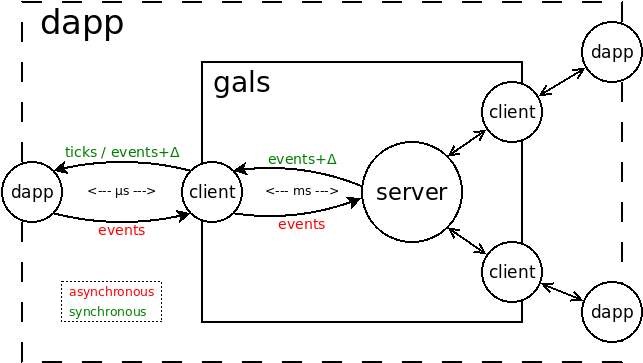
\includegraphics[width=\linewidth]{middleware}
  \caption{
    \label{fig.middleware}
    The architecture of the middleware \emph{gals}.
    A single server synchronizes multiple clients, each connected to a mirrored
    instance of the distributed application.
  }
  %\Description{A woman and a girl in white dresses sit in an open car.}
\end{figure}

The events represent user interactions, such as key presses, which are
unpredictable and need to be communicated with the other instances.
Since instances should be indistinguishable from one another, event sources are
irrelevant.
For instance, if a user presses a key in one instance, the \emph{dapp} behaves
as if all users pressed the same key in all instances simultaneously.
%
Clock ticks represent the rate in which applications are updated, and are
equivalent to frame rates in video playback and games.
For practical purposes, we assume periods in the order of tens of milliseconds
(e.g., 25 milliseconds or 40 frames per second).
An important insight is that clock ticks are predictable inputs and need not to
go through the server.
This results in no delay between the \emph{dapp} and the client since
interprocess communication takes negligible time (i.e., in the order of a few
microseconds).
Unlike sporadic mechanical user input, clock ticks cannot tolerate considerable
delays without going unnoticed by humans.
%
Clock ticks and delayed events constitute the unique synchronous timeline
shared by all instances of the \emph{dapp}, allowing them to manifest identical
behavior.
Figure~\ref{fig.timeline} is an example of a timeline with asynchronous events
that are synchronized with a delay.
As detailed in Section~\ref{sec.gals}, the middleware ensures that all
instances receive the same timeline.

\begin{figure}[t]
{\scriptsize
\begin{verbatim}
Tick    Event    Async
----    -----    -----
0000      0
0025      0      --> user presses key (1) and mouse (2)
0050      0
0075      0      --> user presses key (1)
0100      0
0125      1  <-- key is synchronized after delay
0150      0
0175      2  <-- mouse is synchronized after delay
0200      1  <-- key is synchronized after delay
0225      0
0250      0
....     ...
\end{verbatim}
}
  \caption{
    \label{fig.timeline}
    Example of a synchronized timeline of inputs shared by all instance of the
    \emph{dapp}.
    Ticks are \emph{25ms} apart (40 FPS).
    Asynchronous events are synchronized with a delay.
    Note that delay is unpredictable but event order within each source
    instance is preserved.
  }
\end{figure}

%As detailed in Section~\ref{sec.gals}, the delta delay for user input is the
The delta delay for user input is the maximum network round-trip time
considering all clients.
We deliberately assume unbounded network delay to augment the scope of
applications.
Another concern is the rate of input generation in the instances.
As an example, tracking the mouse position will inevitably flood the network
with packets and make the application unresponsive.
For these reasons, the viability of applications depends on
    (i) the acceptable delay in the user input,
    (ii) the nature and rate of inputs, and
    (iii) the maximum network latency.

The code for an actual \emph{dapp} is the same for all instances and uses a
standard event-driven API with only four commands:
\begin{itemize}
\item \texttt{connect(port,fps)}:        \\Connects with the local client in the given port and desired FPS.
\item \texttt{disconnect()}:             \\Disconnects with the local client.
\item \texttt{(now,evt) = gals\_wait()}: \\Waits for the next input carrying a timestamp and event id.
\item \texttt{gals\_emit(evt)}:          \\Emits the given asynchronous input.
\end{itemize}
Figure~\ref{fig.skel} shows the skeleton of an application.
The commands \texttt{connect} and \texttt{disconnect} are only required once to
enclose the application logic.

\begin{figure}[t]
{\scriptsize
\begin{verbatim}
01  fun dapp (port: Int) {
02     gals_connect(port,40)          // connects to client at 40 FPS
03     while (true) {                 // main event loop
04        val (now,evt) = gals_wait() // awaits input (every 25ms)
05        switch (evt) {              // reacts to input
06           ...gals_emit(nxt)...     //   possibly generates inputs
07           ...break loop...         //   possibly terminates
08        }
09     }
10     gals_disconnect()              // disconnects with the client
11  }
\end{verbatim}
}
  \caption{
    \label{fig.skel}
    The skeleton of a \emph{dapp} is a main loop that waits synchronous and
    emits asynchronous events.
  }
\end{figure}

Figure~\ref{fig.timeline}~and~\ref{fig.skel} with the timeline and the program
related as follows:
The application initially blocks at \emph{line 4} waiting for an input.
According to the timeline, the first input happens at \emph{tick 0} and
\emph{event 0} (no event).
In the second iteration \emph{tick 25}, the application emits events \emph{1}
and \emph{2} asynchronously at \emph{line 6}.
Only after a few ticks, these events are synchronized and awake \emph{line 4}
in subsequent ticks.
The main event loop is coded like a standard local event-driven application as
intended.

\section{Local Synchronous Programming}
\label{sec.sync}

In the synchronous programming model~\cite{sync}, a program executes in
locksteps (or logical ticks) as successive reactions to inputs provided by an
external environment.
In our context, the environment represents user interactions, and inputs can be
occasional events, such as a key press, or simply the passage of time.
Since execution is guided from outside, the main advantage of the synchronous
model is that it can record a sequence of inputs and reproduce the behavior of
a program multiple times for reasoning and testing purposes.
A fundamental requirement for synchronous programming, known as the
\emph{synchronous hypothesis}~\cite{hypo}, is to isolate logical ticks from one
another to preserve locksteps and prevent concurrent reactions to inputs, which
would break determinism.
This hypothesis is satisfied if computing reactions is faster than the rate of
external inputs.

An important concern is how to guarantee that isolated reactions are themselves
deterministic and sufficiently fast.
Synchronous languages~\cite{langs} typically restrict the programming
primitives and/or perform static analysis to ensure these properties.
However, since our solution proposes a standard event-driven API targeting
generic programming languages, we assume these properties are ensured
informally.
This may involve coding best practices like avoiding stateful system calls and
time-consuming loops.

\begin{figure}[t]
  \centering
  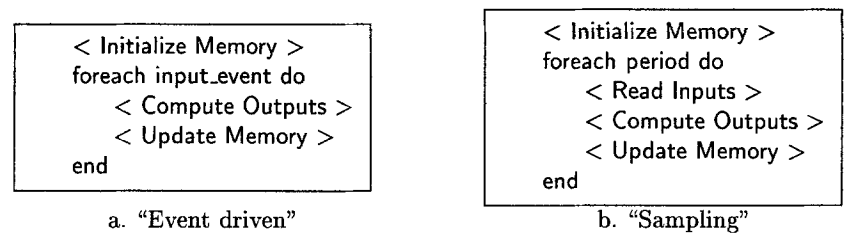
\includegraphics[width=\linewidth]{schemes}
  \caption{
    \label{fig.schemes}
    Equivalent execution schemes for synchronous systems.~\cite{schemes}
    In the first scheme, a change in the environment is designated as an input
    event. 
    In the second scheme, an instant is a predefined time interval in which
    the environment is polled for input events.
  }
\end{figure}

Figure~\ref{fig.schemes} shows two common implementation schemes for
synchronous systems~\cite{schemes}.
In both schemes, a loop iteration updates the state of the memory completely
before handling the next input.
Hence, assuming memory updates are deterministic, the only source of
non-determinism resides in the order of inputs from the environment.
Outputs are events in the opposite direction of inputs and signal the
environment about changes.
They typically represent actuators (as opposed to input sensors), such as the
screen or printer.

The ``Sampling'' scheme of Figure~\ref{fig.schemes} is very similar to the
\emph{dapp} skeleton of Figure~\ref{fig.skel}:
    \texttt{gals\_connect} specifies the sampling period,
    \texttt{gals\_wait} reads inputs,
    \texttt{gals\_emit} signals the environment back, and
    the \texttt{switch} statement processes the inputs (to update memory).
As a subtle difference, instead of output events, \emph{dapps} emit
asynchronous inputs that are later retrofitted back as synchronous inputs with
a delay, as described in Figure~\ref{fig.middleware}.
As required by the synchronous hypothesis, the sampling period, and
consequently the rate of inputs, must be compatible with the processing speed.

The sampling scheme is also adopted by popular event-driven libraries, such as
\emph{SDL} for computer graphics, and \emph{Arduino} for embedded systems.%
\footnote{\url{www.libsdl.org} and \url{www.arduino.cc}}
This allows for an easier integration of our middleware with practical systems,
and also reinforces how programming distributed versions are similar to their
local counterparts.
Figure~\ref{fig.sdl} is the code for a \emph{dapp} written in SDL to control an
animated rectangle on the screen with the keyboard.%
\footnote{Video of the \emph{dapp} running in two instances: \url{TODO}}
The code structure follows the synchronous implementation scheme with evident
sections to initialize memory (\emph{ln. 4--8}), read inputs in a loop
(\emph{ln. 11--13}), update memory (\emph{ln. 15--28}), and compute outputs
(\emph{ln. 30--31}).
As mentioned above, the outputs are actually asynchronous inputs, which are
expanded in Figure~\ref{fig.xxx} and discussed further.
The rectangle starts at position \texttt{(10,10)} with no movement
\texttt{vx=vy=0} (\emph{ln. 7--8}).

Except for the hidden xxx, the app is ... det, etc

\begin{figure}[t]
{\scriptsize
\begin{verbatim}
01  int main (void) {
02    gals_connect(port, 40); // 25ms ticks
03
04    SDL_Init(SDL_INIT_VIDEO);                 ---\
05    SDL_Window*   win = SDL_CreateWindow();      |
06    SDL_Renderer* ren = SDL_CreateRenderer(win); |> Initialize
07    int x=10, vx=0; // position and              |    Memory
08    int y=10, vy=0; // speed multipler        ---/
09
10    while (1) {
11      uint64_t now;                           ---\
12      uint32_t evt;                              |> Read Inputs
13      gals_read(&now, &evt);                  ---/
14
15      SDL_SetRenderDrawColor(ren, WHITE);     ---\
16      SDL_RenderClear(ren); // clear screen      |
17      SDL_Rect r = { x, y, 10, 10 };             |
18      SDL_SetRenderDrawColor(ren, RED);          |
19      SDL_RenderFillRect(ren, &r); // draw rect  |
20      switch (evt) { // 5px/40fps -> 200 px/s    |
21        case 0: { x+=5*vx; y+=5*vy; break; }     |> Update Memory
22        case 1: { vx=-1; vy=0; break; }          |
23        case 2: { vx= 1; vy=0; break; }          |
24        case 3: { vy=-1; vx=0; break; }          |
25        case 4: { vy= 1; vx=0; break; }          |
26        case 5: { vy= 0; vx=0; break; }          |
27      }                                          |
28      SDL_RenderPresent(ren);                 ---/
29
30      // emit asynchronous inputs             ---\  Compute Outputs
31      ... gals_emit(evt) ...                  ---/
32    }
33
34    gals_disconnect();
35    return 0;
36  }
\end{verbatim}
}
  \caption{
    \label{fig.skel}
    The skeleton of a \emph{dapp} is a main loop that waits synchronous and
    emits asynchronous events.
  }
\end{figure}

\begin{comment}
\begin{lstlisting}[
  xleftmargin=1em,
  numbers=left,
  basicstyle=\ttfamily\scriptsize,
  float=t,
  caption={Synchronous application that turns the LED on whenever the button
           is pressed and off whenever it is unpressed.},
  label={lst.gpio.sync},
  escapechar=\%,
]
#include "gpio.ceu"      // GPIO driver
emit PIN_13(low);
loop do
    var high/low v = await PIN_02;
    emit PIN_13(v);
end
\end{lstlisting}
\end{comment}

- SDL stub would allow for ...

how development is similar.

for interaction
with


... TODO ...

\begin{comment}

Environment replicated in the clients

- rate of inputs, time to compute the memory (gancho com "this hypothesis is satisfied if..." acima)
- link to timeline and dapp code

In synchronous systems, communication is instantaneous. The zero-
delay property of the synchronous hypothesis guarantees that no time elapses
between event announcement and receiving. Also, as communication is via
broadcast, all systems parts share the same information all the time. These two
characteristics make global data consensus another property of synchronous
systems.
The first scheme of implementation resembles the main-loops of event-
driven programming in traditional languages. In fact, event-driven program-
ming is the commonest way of programming synchronous systems. Among the
common problems with this pattern are programming with control inversion
and the lack of stack for managing state [von Behren]. We can consider that
event-driven programming is a low-level way of programming synchronous sys-
tems, not much different than dealing with interrupt handling in hardware.
\end{comment}

\begin{comment}
Synchronous: reactions run atomically and to comple-
tion on each line of execution, i.e., there’s no implicit
preemption or real parallelism.

Synchronous: reactions run atomically and to com-
pletion on each line of execution, i.e., there’s no
implicit preemption or real parallelism.

The synchronous execution model of Céu dictates
that reactions to input events are atomic and that in-
coming events are never lost, which we refer to as the
atomicity and responsiveness properties, respectively.

They rely on
the synchronous hypothesis which states that programs take no time to produce
outputs when reacting to inputs. The precise notion of time in these languages
is suitable for programming operations that should be performed respecting a
given timing constraint, which are common case in multimedia.
\end{comment}

\section{Distributed GALS Architecture}
\label{sec.gals}

\begin{comment}
- freezes make clients to fall behind in time
- testar isso com um cliente lazy

- fazer ajuste de tempo dinamico
- qvento de sync a cada segundo? (ou multiplo do RTT)


The ``Globally-Asynchronous Locally-Synchronous Architecture (GALS)''
integrates multiple independent synchronous processes as a single distributed
application.

  shows that ... but local
With distribution, communication timing is asynchronous because communication
latency takes a non-negligible time and breaks the synchronous hypothesis.

Test locally in one instance is the same as N instances in M machines
What about in realtime
- a perfect mirror, cannot distinguish
- high-level vs low-leve events, semantic events
    - more abstract solves both problems (delay and rate)
- clear/sound properties to reason
- Events: single application, multiple views, may restrict events per node

Concurrent programs in non-deterministic languages are notoriously hard to prove correct and have led to well-known disasters.
\end{comment}

\section{Evaluation}
\label{sec.eval}

% - asymmetric, different view, multiple inputs

\section{Related Work}
\label{sec.related}

\begin{comment}
Asynchronous languages and models:

Derflow: distributed deterministic dataflow programming for erlang
Erlang implements a message-passing execution model in which concurrent processes send each other messages asynchronously. This model is inherently non-deterministic: a process can receive messages sent by any process which knows its process identifier, leading to an exponential number of possible executions based on the number messages received.
We propose a new execution model for Erlang, ''Deterministic Dataflow Programming'', based on a highly available, scalable single-assignment data store implemented on top of the riak\_core distributed systems framework.

Deterministic Actors
While actors provide a more disciplined model for concurrency than threads, their interactions, if not constrained, admit nondeterminism.
 We describe “reactors,” a new coordination model that combines ideas from several of the aforementioned approaches to enable determinism while preserving much of the style of actors.

Deterministic replay of distributed Java applications
Execution behavior of a Java application can be nondeterministic due to concurrent threads of execution, thread scheduling, and variable network delays. This nondeterminism in Java makes the understanding and debugging of multi-threaded distributed Java applications a difficult and a laborious process.
It is well accepted that providing deterministic replay of application execution is a key step towards programmer productivity and program under-standing.
Towards this goal, we developed a replay framework based on logical thread schedules and logical intervals.

Synchronous languages and models:

A Programming Model for Time-Synchronized Distributed Real-Time Systems
Discrete-event (DE) models are formal system specifications that have analysable deterministic behaviors. Using a global, consistent notion of time, DE components communicate via time-stamped events.
In this paper, we extend DE models with the capability of relating certain events to physical time.
Our technique relies on having a distributed common notion of time, known to some precision.
\end{comment}

\section{Conclusion}
\label{sec.conclusion}

\bibliographystyle{ACM-Reference-Format}
\bibliography{rebls-21}

\end{document}
\endinput
